\documentclass[11pt]{article}
\usepackage{geometry}                % See geometry.pdf to learn the layout options. There are lots.
\geometry{letterpaper}                   % ... or a4paper or a5paper or ... 
%\geometry{landscape}                % Activate for for rotated page geometry
%\usepackage[parfill]{parskip}    % Activate to begin paragraphs with an empty line rather than an indent
\usepackage{graphicx}
\usepackage{color}
\usepackage{amssymb}
\usepackage{epstopdf}
\usepackage{sectsty}
\usepackage[hyphens]{url}  %% be sure to specify the option 'hyphens'
\DeclareGraphicsRule{.tif}{png}{.png}{`convert #1 `dirname #1`/`basename #1 .tif`.png}

\title{Drake-Cullen-Academic-Integrity}
\author{Drake Cullen}
%\date{}                                           % Activate to display a given date or no date

\begin{document}
%\maketitle
%\section{}
%\subsection{}
\begin{minipage}{\linewidth}% to keep image and caption on one page
\centering
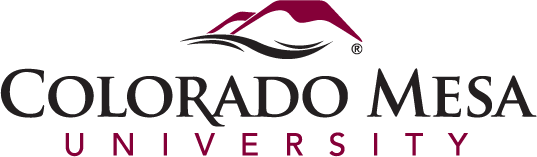
\includegraphics[keepaspectratio=true,scale=0.35]{CMU.png}
\end{minipage}
\section*{ \centering Academic Integrity}
\subsection*{ \centering By Drake Cullen} 

\vspace{5mm}
 
\tableofcontents

\clearpage

\section{Introduction}
Academic integrity is the cornerstone for a successful life. Students who practice integrity inside the classroom carry the attributes into the rest of their lives; therefore, it is of utmost importance for students to gain a comprehensive knowledge of the topic. Once a student fully grasps the topic, they can practice it's methods in the classroom for the rest of their educational career. Throughout the paper, the development of academic initiatives will be established, and their importance will be discussed. In doing so, the reader will learn how to commit themselves to academic excellence. 
\section{Four Initiatives}
Ensuring academic integrity on a college campus is a difficult task. You have a large body of students from different backgrounds who are away from home for the first time. To make matters worse, the rise of technology has further complicated matters by making it easier for students to cheat. To address these issues, four initiatives can be introduced. The four initiatives are: create assessments with larger test pools, have periodic check-ins for larger projects, clearly define policies in the syllabus, and implement software to check for plagiarism.  

One area where students tend to commit academic violations occurs when taking exams. Students will gain answers from students who took the class in the previous year. They may even fake an illness on the day of an exam so that they can get answers from other students. Several steps can be taken to address these concerns. First, exams should have a larger testing pool [1]. Software should be used to randomly select questions from the pool. In doing so, students will all have different exams. This will make it harder to look at your neighbor's test and copy off it. Next, if a professor wants to reuse an exam in the future, students should not be able to take the test home with them. This will prevent future students from getting a copy of the exam before they take it. Finally, an older version of the test (maybe from several years ago) can be given to students who were “sick” on the day of the exam. Taking these actions should help counter cheating on exams.  

A lot of academic dishonesty is sprouted from the fact that students procrastinate. They realize that they won’t have time to complete the project, so they panic and try to get answers. Professors should have check-ins more often on larger projects. These check-ins should be graded to encourage students not to procrastinate. Furthermore, it is easier to check smaller pieces of a project for academic dishonesty than an entire project.   

Another initiative is for Professors to have a detailed section in their syllabus regarding academic integrity. On the first day, the topic should be covered extensively. The severity of violations must be expressed [1]. Finally, software that checks for plagiarism should be implemented in all classes. Any sort of writing, whether it be an essay or code, should be passed through the program. The fear of being caught will detour most students from plagiarizing. Now that initiatives have been established, it is important to look at those who instill academic integrity: role models. 

\section{Role Model}

My older brother Tanner is my role model and the embodiment of academic integrity. He is 25 years old and an alumnus of the Colorado School of Mines where he studied mechanical engineering. Currently, he is working for the patent office. According to Barizsne Hadhazi, the three greatest traits of an ethical person are trustworthiness, honesty, and integrity [2]. Tanner is exceptionally strong in these areas. 

A trustworthy person will consistently be available to help you in a time of need. Anyone who knows my brother will turn to him when they need someone they can rely on. For instance, there was a youth football team called the Mustangs who needed a new coach (Tanner used to play on one of their teams when he was a kid). He didn’t know anyone on the team, but they called him and asked him if he was willing to be their coach. He agreed and didn’t miss a single practice or game. All of the kids on the team loved him.  

As kids, we use to play sports in the house. One of our favorite games to play was dodgeball. One day, we broke our mom's favorite vase with the dodgeball. I was too afraid to tell her, but he told her what happened and apologized. Tanner is one of the most honest people I have ever met. He never tells a lie and will always go out of his way to make things right. 

The last trait of an ethical person is integrity. A kid in Tanner’s elementary school used to wear a mouth guard because his mom was afraid his teeth would get knocked out. The other kids made fun of him for it. My brother was always kind to him, and he would stick up for him when the other students poked fun. Tanner and that kid are still friends to this day. The next section will explore individual's values by diving into their academic integrity. 

\section{Personal Values and Academic Integrity Violations}
You can learn a lot about a student's values by looking into their academic integrity. For instance, students who care about learning will uphold their academic integrity [3]. These students tend to think about academics in the old saying that you play a game like you practice. If you put in the work and practice hard, you are going to play hard when things get tough. On the other hand, if a student is willing to cheat in school, they won’t learn the necessary material to succeed in the real world; therefore, they are more likely to cheat at their job and other aspects of their life. Eventually, this will catch up to them and they will have trouble moving forward  

There are many ways to violate academic integrity. First, is the most obvious one. If you copy or falsify a document in any way, that is a violation. For instance, copying a classmate's homework is an example of this violation The next violation has to do with interfering with another person’s work. If you delete another student’s essay, that is academic dishonesty. Many people may find it surprising, but if you help another student perform academic dishonesty, you are to blame as well. Let's say that your friend hasn’t finished an assignment, so you send them a link to solutions online. You are just as guilty as your friend is. Additionally, any form of cheating in the classroom is a violation of academic integrity. For instance, cheating off your neighbor's exam or looking up answers on a lab computer.  Many classes take attendance for a grade. If you can’t make a class and someone else “attends” for you, that is a violation as well. Furthermore, online software will often grade you on accuracy. If you create multiple accounts so that you can perform more submissions, you are at fault. Finally, any form of prohibited collaboration violates academic integrity. Colorado Mesa University looks to subdue these violations by introducing CMU's learning outcomes. 

\section{Learning Outcomes}
Colorado Mesa University has six different learning outcomes that were developed to promote integrity and achievement. By promoting these learning outcomes, everyone involved with CMU hopes to bring students closer to the community and institution. Not only do students benefit from these outcomes, everyone in the community as well as those who may meet the students in the future will be better off because of these learning outcomes.  

The first learning outcome has to do with the application of learning. By interacting with learning environments, students will gain a great deal of information that can be applied to their educational degree as well as the rest of their lives. Next, students should develop critical thinking skills. In doing so, they will be able to make educated decisions in the future. Students will learn to evaluate all possibilities and not make rash decisions. The third learning outcome claims that students should continually build on their identity. They will become stronger individuals with greater moral values. The next important attribute is to learn how to work with others. At CMU, students will work on their collaboration and leadership skills. These skills are vital to accomplishing large projects that require teamwork. In addition to working with others, students must learn how to give their time and their money to other less fortunate people. We must acknowledge the fact that we are lucky to be where we are today. By giving back, other people will be able to have the opportunities that we have been given. Finally, students will combine all their skills so that they can live a successful and purposeful life. This success starts with the ability to accurately cite sources. 

\section{Citing Sources}
There are many reasons that citing work is important in the academic environment. For starters, the author should be granted credit for their work. It is easier to see the importance of this point if you switch roles. For instance, say that you spent time performing research or looking into a new algorithm. After many years, you may post your findings online for others to investigate. If someone else found your work and took credit for it, you would be rather upset. Try to remember this example whenever you are citing sources.  

Furthermore, by citing sources, interested readers can learn more about the topic you are presenting. Oftentimes, you only select a small piece of a larger work to discuss; therefore, the interested reader can learn more from the cited source [4]. One example of this can be seen if you use Wikipedia. The content will be summarized, but you can explore the links at the bottom to get a more comprehensive overview of the topic. Finally, citing sources preserves your academic integrity.  

In the real world, plagiarism can be much worse than a zero on an assignment. For instance, plagiarism is likely to result in termination from your job. If you are going to give a presentation and you copy one from online, it will be obvious that the content was copied because you won’t know the content well. Afterward, you will be reprimanded by your boss and there is a high chance that you will be fired. In another example, if you steal someone else’s code, there could potentially be a lawsuit. Say that you take code from online to create an AI in your video game. If your game becomes popular and makes a good deal of money, the creator of the AI will be rather upset with you. They will try to find a way to get back at you. The next key idea to understand is the importance of reporting an academic integrity violation. 

\section{Reporting Violations}
Not reporting an academic integrity violation is as bad as committing a violation. By not reporting the incident, you are hurting everyone around you. The student that committed the violation isn’t learning the material, your classmates' grades may suffer because the scoring curve may be affected, and the teacher isn’t able to properly fulfill their job. If you don’t report the violation, you are saying that it is alright to be academically dishonest; therefore, your integrity will be greatly decreased. Sadly, in a survey of students, only 35.7 percent said that they would report academic dishonesty [5].  

Reporting a violation can be rather difficult if your friend commits it because nobody wants to lose a friend. Although it is rather difficult to report them, in the long run, you are helping them out. You are forcing your friend to learn the content rather than cheating, so they will do better in the future. Additionally, students may find it difficult to report a violation if they may think that they could get into trouble. This line of thought is prevalent in many different scenarios in life. Oftentimes, people who are drinking and have a friend in bad condition are too scared to call for help because they don’t want to get in trouble. In the end, you have to put the fear aside for the greater good. Report those who violate academic integrity (even those who collaborate on homework). 

\section{Collaboration on Homework}
Homework is necessary for students to fully understand the topics presented in the classroom, and many other factors contribute to its importance. Mainly, homework teaches responsibility and makes individuals set and achieve goal [6]. Every student should complete their assignments so that they learn these skills.  

Professors don’t like collaboration on homework because kids tend to take the idea of collaboration and stretch it. Students will claim that they are collaborating on homework, but they will really divide the sections, each complete a few, then share the results. Additionally, certain students will wait until the homework is almost due to looking at it. They will realize that they don’t have time to complete the assignment, so they will pester someone else for help. Usually, they will find another student who is willing to help, and they will manage to get the answers from that person. We learn best when we struggle with a concept and are forced to figure it out. Usually, there are challenging problems on a homework assignment that are meant to make students think. If collaboration is allowed, a few students will figure out the problem and the others will take their answers. This leads to the idea of whether or not it is favorable to get help from others on an assignment or exam. 

\section{Receiving Help on Homework}
Receiving help on an assignment can be advantageous when you have spent a considerable amount of time on the problem. Sometimes, you will get so lost in the problem that you begin to miss obvious elements. At this point, a nudge in the correct direction is rather beneficial. Furthermore, if someone acts as a mentor to you, the relationship is two ways. They may help you solve the problem, but you could introduce them to new ways of thinking and form a friendship [7]. On a separate note, if you are helped on an exam, you could receive a high enough score to pass the class. In doing so, you would save money by not having to retake the class  

On the other hand, if someone helps you, there is a good chance that you don’t understand the concept. You will work off their ideas to get the assignment done. The other person may feel trapped in helping you in the future and it will be a time sink for them. Furthermore, they are risking their academic integrity to help you. Regarding receiving help on an exam, you are only setting yourself up for failure in the future  

In conclusion, helping others on an assignment or exam is more harmful than helpful for both parties. In the future, if I am stuck and in need of help, I will reach out to my professor. If I am asked to help someone else, I will encourage them to work on the problem a bit longer and reach out to the professor if they are still stuck 

\section{Conclusion}
Strong academic integrity is the key to living a fulfilling life. Luckily, living a life of integrity is not that difficult of a task. As long as you put effort into your work and avoid taking the easy way out, you will be successful in the pursuit of academic excellence. 

\clearpage

\begin{thebibliography}{1}

\bibitem{impj} ‘Course Design, Monitoring Help Ensure Academic Honesty’ (2005) {\em Online Classroom}, pp. 1–3. Available at: \url{ http://search.ebscohost.com.ezproxy.coloradomesa.edu/login.aspx?direct=true\&db=aph\&AN=15536927\&site=eds-live\&scope=site} (Accessed: 25 August 2021). 

  \bibitem{impj} Barizsne, H. (2019) ‘What Is an Ethical Leader Like? A Study Based on Business Students’ Opinions’, {\em Annals of    the University of Oradea, Economic Science Series}, 28(2), pp. 231–240. Available at:  \url{http://search.ebscohost.com.ezproxy.coloradomesa.edu/login.aspx?direct=true\&db=bth\&AN=141445397\&site=eds-live\&scope=site} (Accessed: 25 August 2021). 

\bibitem{impj}
Miller, A., Shoptaugh, C. and Wooldridge, J. (2011) ‘Reasons Not to Cheat, Academic-Integrity Responsibility, and Frequency of Cheating’, {\em Journal of Experimental Education}, 79(2), pp. 169–184. doi: 10.1080/00220970903567830. 


\bibitem{impj} ‘Identifying Parts of a Citation: Why Citing Sources is Important’ (2020) {\em University of Nebraska}. Available at: \url { https://guides.library.unk.edu/c.php?g=710678\&p=5051044} (Accessed: 25 August 2021). 

\bibitem{impj} Simon, Christopher A. et al. (2004) ‘Gender, student perceptions, institutional commitments and academic dishonesty: who reports in academic dishonesty cases?’, {\em Assessment \& Evaluation in Higher Education}, 29(1), pp. 75–90. doi: 10.1080/0260293032000158171. 

\bibitem{impj} Mayoh, L(2017) ‘The importance of homework for kids’, {\em Centralian Advocate}, 14 July, p. 44. Available at: \url {http://search.ebscohost.com.ezproxy.coloradomesa.edu/login.aspx?direct=true\&db=n5h\&AN=9X9CAVNEWSMMGLSTRY000296420293\&site=eds-live\&scope=site} (Accessed: 25 August 2021). 

  \bibitem{impj} Beaudette, D. (2013) ‘Asking for Help: The Key to Career Success’, {\em Educational Horizons}, 92(1), pp. 12–15. Available at: \url{http://search.ebscohost.com.ezproxy.coloradomesa.edu/login.aspx?direct=true\&db=edsjsr\&AN=edsjsr.42927202\&site=eds-live&scope=site} (Accessed: 25 August 2021). 











 \end{thebibliography}

\end{document}  